%%%%%%%%%%%%%%%%%%%%%%%%%%%%%%%%%%%%%%%%%%%%%%%%%%%%%%%%%%%%%%%%%%%%%%%%%%%%%%%%%%%%%%%%%%%%%%%
%Plantilla: para la realizaci�n de informes.
%Curso:     Simulaci�n estad�stica.
%Profesor:  Johann A. Ospina.
%%%%%%%%%%%%%%%%%%%%%%%%%%%%%%%%%%%%%%%%%%%%%%%%%%%%%%%%%%%%%%%%%%%%%%%%%%%%%%%%%%%%%%%%%%%%%%%


%Establece el tipo de documento (art�culo), tama�o de letra (10pt) a una columna.
\documentclass[letterpaper,12pt,onecolumn,titlepage]{article} 
 
 
% Cargar paquetes
\usepackage{verbatim}
\usepackage{mathrsfs}
\usepackage{amsmath}
\usepackage{amssymb}
\usepackage{subfigure}
\usepackage{ucs}
\usepackage[latin1]{inputenc}
\usepackage[spanish]{babel}
\usepackage{fontenc}
\usepackage{graphicx}
\usepackage{anysize}
\usepackage{fancyhdr}
\usepackage[comma,authoryear]{natbib}
\usepackage{url} %paquete para definir url
\usepackage{hyperref}  %hipervinculos

%Estilo de la p�gina
\pagestyle{fancy}

%Establecer el margen
\marginsize{1.5cm}{1.5cm}{1.5cm}{1.5cm}
\setlength{\headheight}{13.1pt}


% Portada
\title{
    \textbf{Simulaci�n de la Probabilidad}\
    ~\\{Simulaci�n Estad�stica}   
    }
\author{
    {Diana Carolina Arias Sinisterra Cod. 1528008}
 ~\\{Cesar Andres Saavedra Vanegas Cod. 1628466}}






\date{
     \textbf{Universidad Del Valle}\   
    ~\\{Facultad De Ingenieria}
    ~\\{Estadistica}
    ~\\{Febrero}
    ~\\{2018}}
 
 
 
\decimalpoint %Poner punto decimal
 
\begin{document}
 
% Se aplica el formato a las p�ginas. Se despliegan: portada e �ndices de materias, figuras y tablas
\renewcommand{\listtablename}{}
\renewcommand{\tablename}{Tabla}
\maketitle
\setcounter{page}{2}

%\thispagestyle{empty}
%\newpage


\thispagestyle{empty}

\newpage
\fancyhead{}
\fancyfoot{}
 
% Encabezado y pie de pagina
\lhead{Simulaci�n Estad�stica}
\lfoot{Universidad Del Valle}
\rfoot{\thepage}

% Estilo de la bibliograf�a
\bibliographystyle{apalike}
 
% Desarrollo de los contenidos del documento

\section{Situaci�n 1}
~\begin{itemize}
\item\textbf {Parte A:} En la situaci�n 1 se plantea un escenario para el cual se tiene una poblaci�n de 100 chips de memoria, de los cuales 90 se encuentran en buen estado y 10 da�ados. Debemos escoger 5 entre los 100 para su uso, por medio del software estad�stico R usamos la funci�n "sample" para dar una aproximaci�n del valor de la probabilidad de que los 5 chips sean buenos. 
~\\ Mediante la simulaci�n se logra obtener como resultado aproximado una probabilidad de 0.61 de que los 5 chips escogidos de manera aleatoria para reparar la computadora sean buenos.  

\item\textbf {Parte B:} Tomando como base los resultados obtenidos en la Parte A. se propone utilizar una forma alterna para seleccionar los chips y de esta manera calcular la probabilidad y que permita obtener un resultado mucho mas fiel a la realidad y a lo mostrado en el punto anterior. Para los cual decidimos usar la distribuci�n Hipergeometrica para realizar dicha selecci�n con un mejor ajuste obteniendo de esta forma una probabilidad de 0.5837.   
\end{itemize}
 
\section{Situaci�n 2}
~\begin{itemize}
\item\textbf {Parte A:} Para la situaci�n 2, contamos con un problema matem�tico denominado como "La paradoja del cumplea�os" en el cual se plantea encontrar la probabilidad de que dos o mas personas tengan la misma fecha de cumplea�os. Para verificar dicha hip�tesis en la cual a mayor numero de personas en un cuarto mayor es la probabilidad de coincidencia se realizo una simulaci�n y los resultados se presentan mediante las siguientes gr�ficas.  

\begin{figure}[!h]
    \begin{center}
        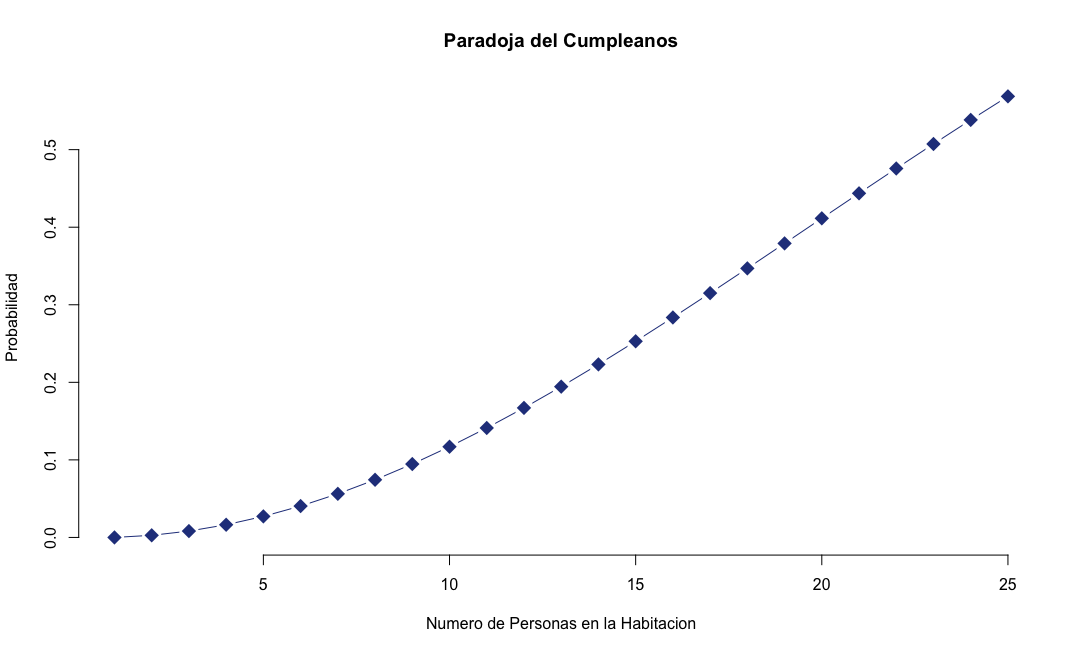
\includegraphics[width=10cm]{Figuras/Rplot02.png}
        \caption{Probabilidad de coincidencia para 25 personas}
        \label{fig:Densidad}
    \end{center}
\end{figure}

\pagebreak
~\\ Destacar que a medida que el numero de personas en la habitaci�n se incrementa la probabilidad de encontrar coincidencia es mayor, algunas de estas probabilidades se muestra mediante la tabla:
\begin{center}
\begin{tabular}{|c|c|c|c|c|}
\hline 
\rule[-1ex]{0pt}{2.5ex}  Individuos & Probabilidad  \\ 
\hline 
\rule[-1ex]{0pt}{2.5ex} 0 & 0.000  \\ 
\hline
\rule[-1ex]{0pt}{2.5ex} 5 & 0.02713  \\  
\hline 
\rule[-1ex]{0pt}{2.5ex} 15 & 0.2529 \\ 
\hline 
\rule[-1ex]{0pt}{2.5ex} 25 & 0.5686  \\ 
\hline 
\end{tabular} 
\end{center}

\item\textbf {Parte B:} 
\end{itemize}
 
\section{Situaci�n 3}
\section{Situaci�n 4}
\section{Situaci�n 5}
\section{Situaci�n 6}
\section{Situaci�n 7}
\section{Situaci�n 8}

\pagebreak\section{Scripts}

\begin{verbatim}
\end{verbatim}

\end{document}








